\chapter{序論}
こんな感じで章ごとにファイル分けるといいよ


\section{章立の際の注意点}
documentclassがjbookだからchapterが章でsectionが節.ipsjと違うので注意.


\section{BibTeXの使い方}

bibファイルに情報を追加することで,勝手に参考文献リストを作ってくれる.本文中で参照していない(citeを使っていない)文献については,bibファイルに記述されていても参考文献リストに出力されないので注意\footnote{参照されているか否かに関わらず,bibファイルに記述されている文献リストを全て参考文献として出力するコマンドもある}.

bibファイルを使いたい場合,bibファイルもコンパイルする必要がある.環境によって差異はありそうだが,まずいつも通りLaTeXを実行し,pBibTeXを実行した後,またLaTeXに2度かける.もっといい方法がありそうだが,とりあえず合計4度のコンパイルをする.参考文献関係の箇所で更新がない限り,通常のコンパイルで問題はない.

以下は,BibTeX情報を取得する方法である.


\begin{figure}[h]
	\begin{center}	
		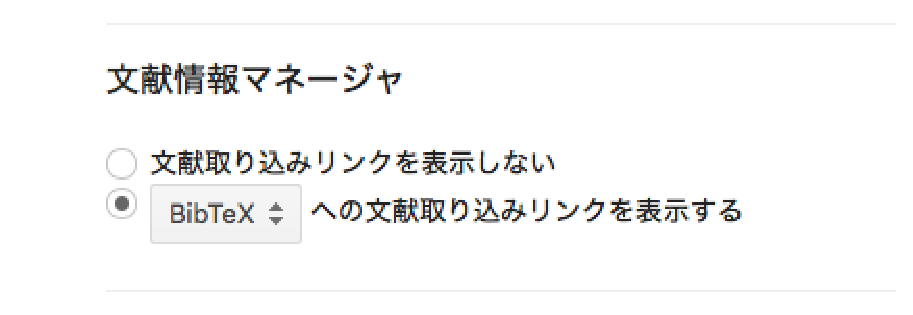
\includegraphics[width=\linewidth]{img/setting.eps}
		\caption{Google Scholarの設定}
		\label{fig:setting}
	\end{center}
\end{figure}


Google Scholarから簡単に取得できる.まずはBibTeXを取得できるように,Google Scholarの「設定」から変更する(\figref{fig:setting}).


\begin{figure}[h]
	\begin{center}
		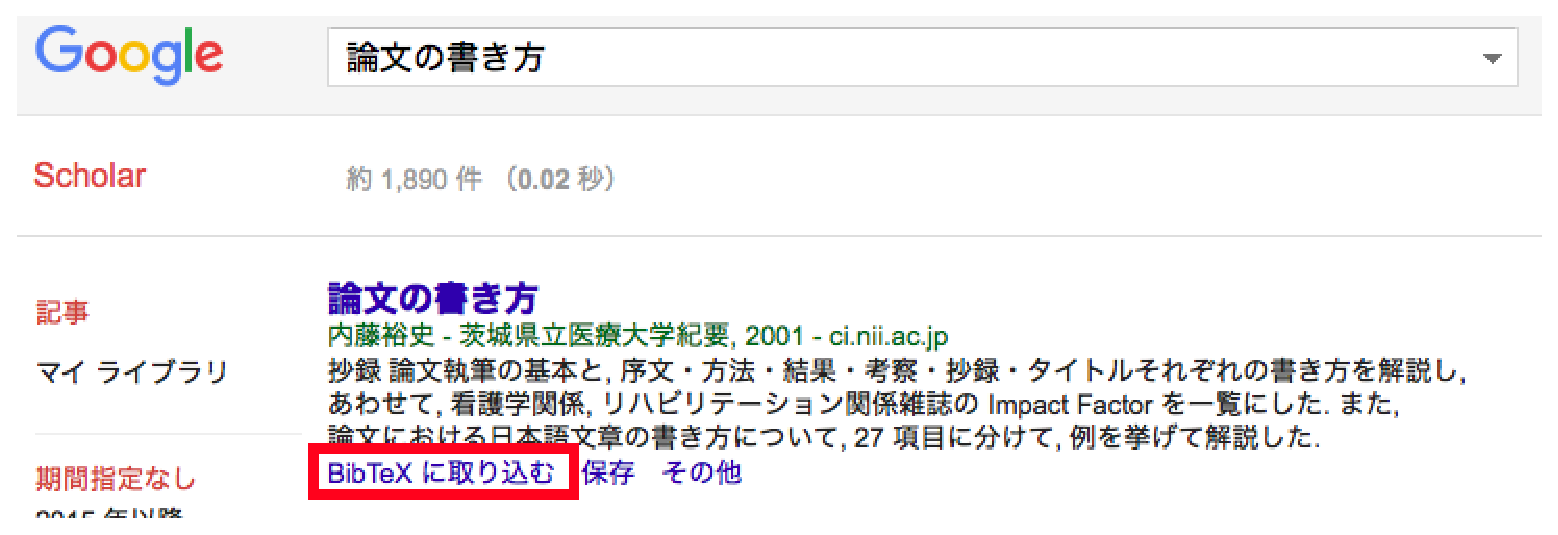
\includegraphics[width=\linewidth]{img/search.eps}
		\caption{BibTeX情報の取得}
		\label{fig:search}
	\end{center}
\end{figure}


そしたら,通常どおり検索をする.検索結果一つ一つに「BibTeXに取り込む」というリンクが表示されるようになっている(\figref{fig:search}).


\begin{figure}[h]
	\begin{center}
		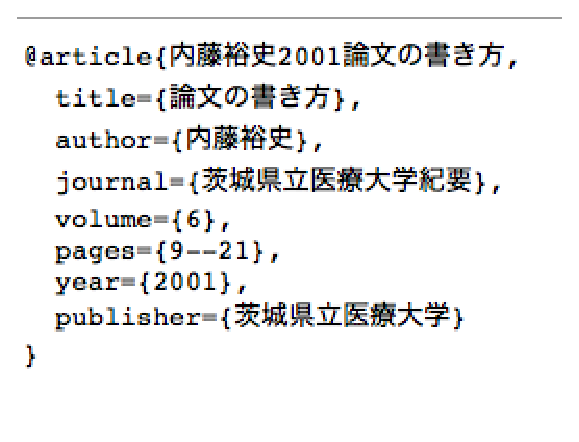
\includegraphics[width=0.5\linewidth]{img/result.eps}
		\caption{BibTeX情報の例}
		\label{fig:result}
	\end{center}
\end{figure}


リンクをクリックすればBibTeX情報が表示される(\figref{fig:result}).これをbibファイルに貼り付けていく.この論文を参照するとこんな感じになる\cite{内藤裕史2001論文の書き方}.「内藤裕史2001論文の書き方」の部分が参照するために必要な箇所.ちなみにこの方法でGoogle ScholarからBibTeX情報を取得すると,おかしい部分があったりするので,適宜手動で修正する.